% Options for packages loaded elsewhere
\PassOptionsToPackage{unicode}{hyperref}
\PassOptionsToPackage{hyphens}{url}
%
\documentclass[
]{article}
\title{Análisis de viabilidad poblacional: Population Viability
Analysis}
\author{BIOL4558}
\date{Agosto 2021}

\usepackage{amsmath,amssymb}
\usepackage{lmodern}
\usepackage{iftex}
\ifPDFTeX
  \usepackage[T1]{fontenc}
  \usepackage[utf8]{inputenc}
  \usepackage{textcomp} % provide euro and other symbols
\else % if luatex or xetex
  \usepackage{unicode-math}
  \defaultfontfeatures{Scale=MatchLowercase}
  \defaultfontfeatures[\rmfamily]{Ligatures=TeX,Scale=1}
\fi
% Use upquote if available, for straight quotes in verbatim environments
\IfFileExists{upquote.sty}{\usepackage{upquote}}{}
\IfFileExists{microtype.sty}{% use microtype if available
  \usepackage[]{microtype}
  \UseMicrotypeSet[protrusion]{basicmath} % disable protrusion for tt fonts
}{}
\makeatletter
\@ifundefined{KOMAClassName}{% if non-KOMA class
  \IfFileExists{parskip.sty}{%
    \usepackage{parskip}
  }{% else
    \setlength{\parindent}{0pt}
    \setlength{\parskip}{6pt plus 2pt minus 1pt}}
}{% if KOMA class
  \KOMAoptions{parskip=half}}
\makeatother
\usepackage{xcolor}
\IfFileExists{xurl.sty}{\usepackage{xurl}}{} % add URL line breaks if available
\IfFileExists{bookmark.sty}{\usepackage{bookmark}}{\usepackage{hyperref}}
\hypersetup{
  pdftitle={Análisis de viabilidad poblacional: Population Viability Analysis},
  pdfauthor={BIOL4558},
  hidelinks,
  pdfcreator={LaTeX via pandoc}}
\urlstyle{same} % disable monospaced font for URLs
\usepackage[margin=1in]{geometry}
\usepackage{color}
\usepackage{fancyvrb}
\newcommand{\VerbBar}{|}
\newcommand{\VERB}{\Verb[commandchars=\\\{\}]}
\DefineVerbatimEnvironment{Highlighting}{Verbatim}{commandchars=\\\{\}}
% Add ',fontsize=\small' for more characters per line
\usepackage{framed}
\definecolor{shadecolor}{RGB}{248,248,248}
\newenvironment{Shaded}{\begin{snugshade}}{\end{snugshade}}
\newcommand{\AlertTok}[1]{\textcolor[rgb]{0.94,0.16,0.16}{#1}}
\newcommand{\AnnotationTok}[1]{\textcolor[rgb]{0.56,0.35,0.01}{\textbf{\textit{#1}}}}
\newcommand{\AttributeTok}[1]{\textcolor[rgb]{0.77,0.63,0.00}{#1}}
\newcommand{\BaseNTok}[1]{\textcolor[rgb]{0.00,0.00,0.81}{#1}}
\newcommand{\BuiltInTok}[1]{#1}
\newcommand{\CharTok}[1]{\textcolor[rgb]{0.31,0.60,0.02}{#1}}
\newcommand{\CommentTok}[1]{\textcolor[rgb]{0.56,0.35,0.01}{\textit{#1}}}
\newcommand{\CommentVarTok}[1]{\textcolor[rgb]{0.56,0.35,0.01}{\textbf{\textit{#1}}}}
\newcommand{\ConstantTok}[1]{\textcolor[rgb]{0.00,0.00,0.00}{#1}}
\newcommand{\ControlFlowTok}[1]{\textcolor[rgb]{0.13,0.29,0.53}{\textbf{#1}}}
\newcommand{\DataTypeTok}[1]{\textcolor[rgb]{0.13,0.29,0.53}{#1}}
\newcommand{\DecValTok}[1]{\textcolor[rgb]{0.00,0.00,0.81}{#1}}
\newcommand{\DocumentationTok}[1]{\textcolor[rgb]{0.56,0.35,0.01}{\textbf{\textit{#1}}}}
\newcommand{\ErrorTok}[1]{\textcolor[rgb]{0.64,0.00,0.00}{\textbf{#1}}}
\newcommand{\ExtensionTok}[1]{#1}
\newcommand{\FloatTok}[1]{\textcolor[rgb]{0.00,0.00,0.81}{#1}}
\newcommand{\FunctionTok}[1]{\textcolor[rgb]{0.00,0.00,0.00}{#1}}
\newcommand{\ImportTok}[1]{#1}
\newcommand{\InformationTok}[1]{\textcolor[rgb]{0.56,0.35,0.01}{\textbf{\textit{#1}}}}
\newcommand{\KeywordTok}[1]{\textcolor[rgb]{0.13,0.29,0.53}{\textbf{#1}}}
\newcommand{\NormalTok}[1]{#1}
\newcommand{\OperatorTok}[1]{\textcolor[rgb]{0.81,0.36,0.00}{\textbf{#1}}}
\newcommand{\OtherTok}[1]{\textcolor[rgb]{0.56,0.35,0.01}{#1}}
\newcommand{\PreprocessorTok}[1]{\textcolor[rgb]{0.56,0.35,0.01}{\textit{#1}}}
\newcommand{\RegionMarkerTok}[1]{#1}
\newcommand{\SpecialCharTok}[1]{\textcolor[rgb]{0.00,0.00,0.00}{#1}}
\newcommand{\SpecialStringTok}[1]{\textcolor[rgb]{0.31,0.60,0.02}{#1}}
\newcommand{\StringTok}[1]{\textcolor[rgb]{0.31,0.60,0.02}{#1}}
\newcommand{\VariableTok}[1]{\textcolor[rgb]{0.00,0.00,0.00}{#1}}
\newcommand{\VerbatimStringTok}[1]{\textcolor[rgb]{0.31,0.60,0.02}{#1}}
\newcommand{\WarningTok}[1]{\textcolor[rgb]{0.56,0.35,0.01}{\textbf{\textit{#1}}}}
\usepackage{graphicx}
\makeatletter
\def\maxwidth{\ifdim\Gin@nat@width>\linewidth\linewidth\else\Gin@nat@width\fi}
\def\maxheight{\ifdim\Gin@nat@height>\textheight\textheight\else\Gin@nat@height\fi}
\makeatother
% Scale images if necessary, so that they will not overflow the page
% margins by default, and it is still possible to overwrite the defaults
% using explicit options in \includegraphics[width, height, ...]{}
\setkeys{Gin}{width=\maxwidth,height=\maxheight,keepaspectratio}
% Set default figure placement to htbp
\makeatletter
\def\fps@figure{htbp}
\makeatother
\setlength{\emergencystretch}{3em} % prevent overfull lines
\providecommand{\tightlist}{%
  \setlength{\itemsep}{0pt}\setlength{\parskip}{0pt}}
\setcounter{secnumdepth}{-\maxdimen} % remove section numbering
\ifLuaTeX
  \usepackage{selnolig}  % disable illegal ligatures
\fi

\begin{document}
\maketitle

{
\setcounter{tocdepth}{2}
\tableofcontents
}
\hypertarget{final-projects}{%
\subsubsection{Final projects:}\label{final-projects}}

Un aviso sobre \href{FINAL_PROJECTS.html}{final projects}. ¡Su PVA de
trabajo y un documento que justifica sus decisiones de modelado vencen
\emph{el viernes 9 de abril }!

\hypertarget{anuxe1lisis-de-viabilidad-poblacional-pva}{%
\subsection{Análisis de viabilidad poblacional
(PVA)}\label{anuxe1lisis-de-viabilidad-poblacional-pva}}

Análisis de viabilidad poblacional: Population Viability Analysis (PVA)
integra todo lo que hemos estudiado hasta ahora y más.

En su nivel más básico, PVA es el \emph{proceso de construcción y
ejecución de un modelo poblacional predictivo formal con el fin de
obtener información sobre el estado de conservación presente y futuro, o
clasificar opciones de gestión alternativas}.

\textbf{P: } ¿El PVA se alinea bien con el paradigma de población
pequeña?

\textbf{P: } ¿El PVA se alinea bien con el paradigma de la población en
declive?

\textbf{P: } ¿Los modelos PVA son siempre estocásticos?

\textbf{P: } ¿Los modelos PVA siempre dependen de la densidad?

\textbf{P: } ¿Los modelos PVA siempre están estructurados por edades?

\textbf{P }: ¿Los modelos PVA son siempre espacialmente explícitos?

\hypertarget{el-proceso-pva-receta-para-pva}{%
\subsubsection{El proceso PVA (¡receta para
PVA!)}\label{el-proceso-pva-receta-para-pva}}

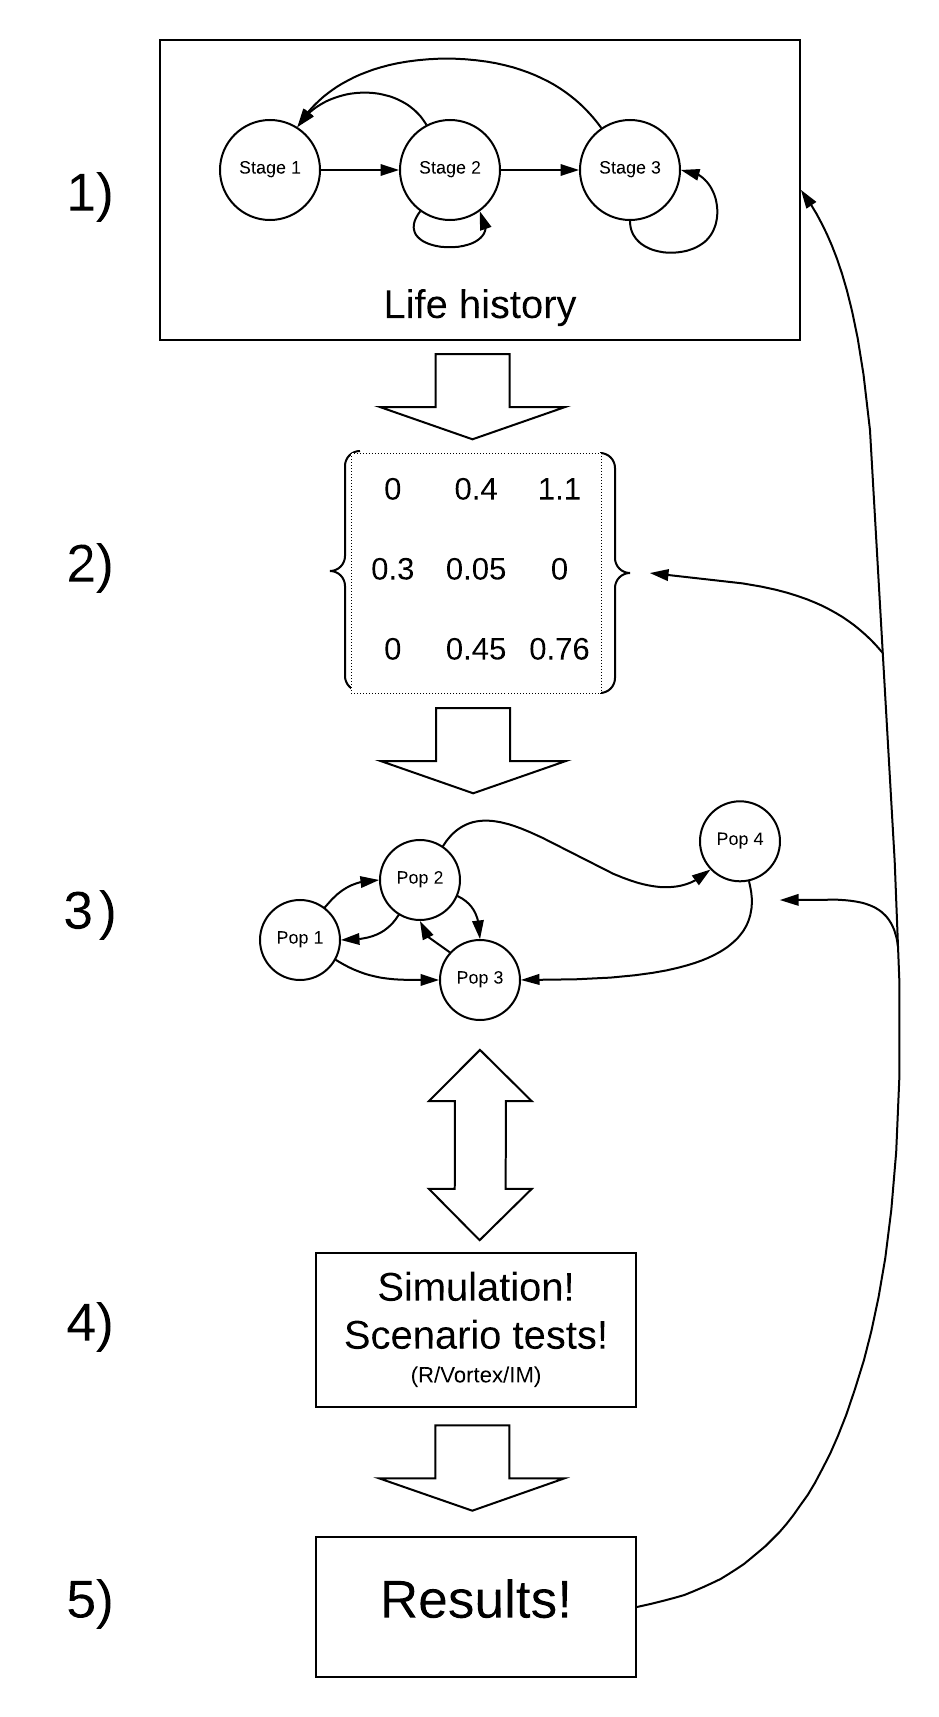
\includegraphics{figures/PVAschematic1.png}

NOTA: El proceso de construcción de un modelo PVA es \textbf{iterativo }
y \textbf{no lineal }.

Por ejemplo, después de ejecutar su modelo (paso 4) y observar los
resultados (paso 5), es posible que se dé cuenta de que el modelo es
totalmente irreal. Esto podría pedirle que retroceda y cambie su modelo
conceptual de la historia de vida (paso 1) y vuelva a parametrizar su
modelo (paso 2).

\hypertarget{paso-1-historia-de-vida}{%
\paragraph{Paso 1: historia de vida}\label{paso-1-historia-de-vida}}

Clase 1: pensamiento sistémico Clase 2: retroalimentación Clase 3:
crecimiento exponencial Clase 4: dependencia de la densidad Clase 5:
efectos allee Clase 6: poblaciones estructuradas por edad Clase 7:
modelos matriciales de población Clase 8: estocasticidad Laboratorios
1,2,3,4,5

El primer paso es conceptualizar la historia de vida de su especie de
interés. Aquí es donde puede armar un diagrama de historia de vida y
pensar en las siguientes preguntas:

\begin{itemize}
\tightlist
\item
  ¿Cuántas etapas de la vida debo incluir?
\item
  ¿Qué etapas de la vida son reproductivas?
\item
  ¿Qué tasas vitales dependen de la densidad?
\item
  ¿Su especie se beneficia de la agregación social? Si es así, ¿hay
  algún efecto de Allee?
\item
  ¿Qué tasas vitales están sujetas a estocasticidad ambiental?
\item
  ¿Qué índices vitales podrían verse alterados por las actividades de
  manejo?
\item
  ¿Existen catástrofes importantes que puedan afectar al sistema?
\end{itemize}

\textbf{P }: ¿hay algún caso en el que \emph{NO } incluyas la
estocasticidad demográfica en tu modelo?

\hypertarget{paso-2-parametrizar-el-modelo-demogruxe1fico}{%
\paragraph{Paso 2: ¡Parametrizar el modelo
demográfico!}\label{paso-2-parametrizar-el-modelo-demogruxe1fico}}

Clase 3: crecimiento exponencial Clase 4: dependencia de la densidad
Clase 5: efecto allee Clase 7: modelos matriciales de población Clase 8:
estocasticidad e incertidumbre Laboratorios 1,2,3,4,5,7

Aquí es donde se adjuntan números reales a las existencias y flujos en
su diagrama de historia de vida conceptual. Recuerde que estos
parámetros son más que solo supervivencia y fecundidad. Es también:

\begin{itemize}
\tightlist
\item
  Variación anual de supervivencia y fecundidad (estocasticidad
  ambiental)
\item
  Abundancias iniciales
\item
  Funciones y parámetros de dependencia de la densidad (incluido K)
\item
  Allee umbrales
\item
  Tamaños y probabilidades del efecto de catástrofe
\item
  Efectos de las acciones de gestión
\item
  Y más\ldots{}
\end{itemize}

{[}¡analogía de la sopa de piedra con la parametrización del modelo!{]}

Paso 3: ¡Estructura espacial!

Clase 13: modelos de metapoblación Clase 14: dinámica fuente-sumidero
Laboratorio 6: modelos de metapoblación

Si desea hacer preguntas espaciales, su modelo debe ser espacialmente
explícito, o al menos considerar la estructura espacial de alguna
manera. Los tipos de preguntas en las que podría pensar incluyen:

\begin{itemize}
\tightlist
\item
  ¿Cuántas poblaciones discretas hay en su metapoblación?
\item
  ¿Las diferentes poblaciones tienen diferentes tasas vitales medias?
  ¿Es probable que algunas poblaciones sean fuentes y otras, sumideros?
\item
  ¿La estocasticidad ambiental ** está espacialmente correlacionada **?
  (¿Es probable que un mal año en una subpoblación sea un mal año en
  todas las subpoblaciones?)
\item
  ¿A qué ritmo se mueven los individuos entre estas poblaciones?
\item
  ¿Se puede mejorar la conectividad mediante la gestión?
\item
  ¿Las tasas de dispersión dependen de la densidad?
\end{itemize}

\hypertarget{paso-4-simular}{%
\paragraph{Paso 4: ¡Simular!}\label{paso-4-simular}}

En los ejercicios de clase, todos los laboratorios

Ya sabe cómo simular poblaciones; puede elegir si tiene sentido utilizar
R, InsightMaker, Vortex o algún otro software o plataforma de
programación para sus simulaciones.

De cualquier manera, puede ser creativo: configure las simulaciones para
que puedan ayudarlo a responder sus preguntas clave de investigación.
Usted tiene el control: ¡puede configurar las simulaciones para que le
brinden los tipos de datos que necesita!

\begin{itemize}
\tightlist
\item
  ¿Qué escenarios quieres probar?
\item
  ¿Cuántas réplicas son suficientes?
\item
  ¿Qué datos necesita almacenar para sus gráficos y análisis?
\end{itemize}

\hypertarget{paso-5-resultados}{%
\paragraph{Paso 5: Resultados}\label{paso-5-resultados}}

Recomiendo usar R para analizar y trazar los resultados de su
simulación. ¡PERO también puede usar Excel e InsightMaker para hacer
gráficos perfectamente buenos!

Por último, debe comprender todas las simulaciones que acaba de
ejecutar.

Hay dos tipos de herramientas de análisis de datos que necesitará para
poder utilizar los resultados de la simulación para responder a sus
preguntas: \textbf{visualización gráfica } y \textbf{análisis
estadístico }.

Estas herramientas (visualización y análisis estadístico) son diversas y
no existe una forma única de visualizar y analizar los resultados de la
simulación. ¡¡Realmente depende de tu pregunta !!

Le daré algunas ideas aquí sobre las representaciones gráficas en el PVA
de demostración, pero recuerde que no está limitado a estas ideas, ¡sea
creativo! Dado que esta clase no es una clase de estadísticas, no
necesariamente espero que haga estadísticas sofisticadas como parte de
su proyecto, pero sus asistentes técnicos y yo podemos trabajar con sus
grupos individualmente para descubrir algunas estadísticas simples que
tengan sentido para su proyecto.

\hypertarget{un-pva-de-demostraciuxf3n-simple}{%
\subsection{Un PVA de demostración
simple}\label{un-pva-de-demostraciuxf3n-simple}}

Para ilustrar algunos de estos conceptos, construyamos un modelo PVA muy
simple en R. Si desea seguir adelante, haga clic {[}aquí{]}
(LECTURA12.R)

Usamos R debido a sus herramientas de visualización flexibles y
poderosas.

\hypertarget{paso-1-conceptualiza-la-historia-de-vida}{%
\subsubsection{Paso 1: conceptualiza la historia de
vida}\label{paso-1-conceptualiza-la-historia-de-vida}}

Para simplificar, ignoremos la estructura de edades por ahora: ¡esto es
solo un modelo de población estocástico simple de una etapa (escalar)!

¡También ignoremos la incertidumbre de los parámetros!

\hypertarget{paso-2-parametrizar}{%
\subsubsection{Paso 2: parametrizar!}\label{paso-2-parametrizar}}

Aquí está la parametrización básica del modelo:

\begin{Shaded}
\begin{Highlighting}[]
\CommentTok{\#install.packages(c(\textquotesingle{}tinytex\textquotesingle{}, dependencies=T))}
\DocumentationTok{\#\#\#\#\#\#\#\#\#\#\#\#\#\#}
\CommentTok{\# Demostración PVA}
\DocumentationTok{\#\#\#\#\#\#\#\#\#\#\#\#\#\#}

\CommentTok{\# PASO 1: conceptualice la historia de vida (estamos modelando esta población como un modelo estocástico simple de una etapa con dependencia de la densidad)}

\CommentTok{\# PASO 2: parametrizar el modelo}

\DocumentationTok{\#\#\#\#}
\CommentTok{\# Parámetros básicos de la historia de vida}
\DocumentationTok{\#\#\#\#}

\NormalTok{R\_max }\OtherTok{\textless{}{-}} \FloatTok{1.15}       \CommentTok{\# Tasa máxima de crecimiento}
\NormalTok{Init\_N }\OtherTok{\textless{}{-}} \DecValTok{51}        \CommentTok{\# Abundancia inicial}
\NormalTok{K }\OtherTok{\textless{}{-}} \DecValTok{175}            \CommentTok{\# CCapacidad de carga}

\DocumentationTok{\#\#\#\#}
\CommentTok{\# Estocasticidad ambiental}
\DocumentationTok{\#\#\#\#}

\NormalTok{SD\_anngrowth }\OtherTok{\textless{}{-}} \FloatTok{0.11}  \CommentTok{\# desviación estándar de la tasa de crecimiento anual}

\DocumentationTok{\#\#\#\#}
\CommentTok{\# Densidad{-}dependencia (modelo de Ricker)}
\DocumentationTok{\#\#\#\#}

\NormalTok{Ricker }\OtherTok{\textless{}{-}} \ControlFlowTok{function}\NormalTok{(prev\_abund)\{       }\CommentTok{\# esta es una función para calcular la abundancia del próximo año {-} incluye estocasticidad env}
\NormalTok{  prev\_abund }\SpecialCharTok{*} \FunctionTok{exp}\NormalTok{(}\FunctionTok{log}\NormalTok{(}\FunctionTok{rnorm}\NormalTok{(}\DecValTok{1}\NormalTok{,R\_max,SD\_anngrowth))}\SpecialCharTok{*}\NormalTok{(}\DecValTok{1}\SpecialCharTok{{-}}\NormalTok{(prev\_abund}\SpecialCharTok{/}\NormalTok{K)))}
\NormalTok{\}}

\DocumentationTok{\#\#\#\#}
\CommentTok{\# Catástrofe}
\DocumentationTok{\#\#\#\#}

\NormalTok{Flood\_prob }\OtherTok{\textless{}{-}} \FloatTok{0.05}      \CommentTok{\# 5\% probabilidad de una gran inundación}
\NormalTok{Flood\_lambda }\OtherTok{\textless{}{-}} \FloatTok{0.25}    \CommentTok{\# 25\% de la población puede sobrevivir a una inundación}
\end{Highlighting}
\end{Shaded}

\hypertarget{step-3-estructura-espacial}{%
\subsubsection{Step 3: estructura
espacial}\label{step-3-estructura-espacial}}

Let's ignore spatial structure! We will learn more about modeling
spatial structure in the next two lectures! ¡Ignoremos la estructura
espacial! ¡Aprenderemos más sobre el modelado de la estructura espacial
en las próximas dos conferencias!

\hypertarget{step-4-simular}{%
\subsubsection{Step 4: ¡simular!}\label{step-4-simular}}

Ahora podemos usar estos parámetros para construir y ejecutar un modelo
PVA simple:

\begin{Shaded}
\begin{Highlighting}[]
\CommentTok{\# PASO 3: agregue estructura espacial (no se aplica aquí)}

\CommentTok{\# PASO 4: ¡simular!}

\DocumentationTok{\#\#\#\#}
\CommentTok{\# Parámetros de simulación básicos}
\DocumentationTok{\#\#\#\#}

\NormalTok{nyears }\OtherTok{\textless{}{-}} \DecValTok{100}     \CommentTok{\# número de años}
\NormalTok{nreps }\OtherTok{\textless{}{-}} \DecValTok{500}      \CommentTok{\# número de réplicas}


\NormalTok{PVAdemo }\OtherTok{\textless{}{-}} \ControlFlowTok{function}\NormalTok{(nreps,nyears,Init\_N,R\_max,K,Flood\_prob,Flood\_lambda)\{}
  \CommentTok{\#browser()}
\NormalTok{  PopArray2 }\OtherTok{\textless{}{-}} \FunctionTok{array}\NormalTok{(}\DecValTok{0}\NormalTok{,}\AttributeTok{dim=}\FunctionTok{c}\NormalTok{((nyears}\SpecialCharTok{+}\DecValTok{1}\NormalTok{),nreps))   }\CommentTok{\# configurar matriz de almacenamiento}
  
  \DocumentationTok{\#\# empezar a recorrer las réplicas}
  
  \ControlFlowTok{for}\NormalTok{(rep }\ControlFlowTok{in} \DecValTok{1}\SpecialCharTok{:}\NormalTok{nreps)\{}
    
    \CommentTok{\# establecer abundancia inicial}
\NormalTok{    PopArray2[}\DecValTok{1}\NormalTok{,rep] }\OtherTok{\textless{}{-}}\NormalTok{ Init\_N     }\CommentTok{\# establecer la abundancia inicial}
    
    \DocumentationTok{\#\#\# recorrer años: loop through years}
    \ControlFlowTok{for}\NormalTok{(y }\ControlFlowTok{in} \DecValTok{2}\SpecialCharTok{:}\NormalTok{(nyears}\SpecialCharTok{+}\DecValTok{1}\NormalTok{))\{}
      \DocumentationTok{\#\#\# estocasticidad y d{-}d}
\NormalTok{      nextyear }\OtherTok{\textless{}{-}} \FunctionTok{max}\NormalTok{(}\DecValTok{0}\NormalTok{,}\FunctionTok{trunc}\NormalTok{(}\FunctionTok{Ricker}\NormalTok{(PopArray2[y}\DecValTok{{-}1}\NormalTok{,rep])))}
      
      \DocumentationTok{\#\#\# catástrofe}
      \ControlFlowTok{if}\NormalTok{(}\FunctionTok{runif}\NormalTok{(}\DecValTok{1}\NormalTok{)}\SpecialCharTok{\textless{}}\NormalTok{Flood\_prob) nextyear }\OtherTok{\textless{}{-}}\NormalTok{ nextyear}\SpecialCharTok{*}\NormalTok{Flood\_lambda}
\NormalTok{      PopArray2[y,rep] }\OtherTok{\textless{}{-}}\NormalTok{ nextyear }
\NormalTok{    \}}
\NormalTok{  \}}
  
  \FunctionTok{return}\NormalTok{(PopArray2)}
\NormalTok{\}}

\DocumentationTok{\#\#\# Run the PVA!}

\NormalTok{Default }\OtherTok{\textless{}{-}} \FunctionTok{PVAdemo}\NormalTok{(nreps,nyears,Init\_N,R\_max,K,Flood\_prob,Flood\_lambda)}
\end{Highlighting}
\end{Shaded}

\hypertarget{step-5-results}{%
\subsubsection{Step 5: results!}\label{step-5-results}}

¡Ahora podemos realizar visualizaciones gráficas y estadísticas que
responden a nuestras preguntas originales!

\hypertarget{visualizaciuxf3n-gruxe1fica}{%
\paragraph{Visualización gráfica}\label{visualizaciuxf3n-gruxe1fica}}

Hay varios tipos de visualizaciones que quizás desee utilizar para sus
modelos PVA:

El primero es mirar la ``nube'' de trayectorias de abundancia. Este es
el mismo tipo de figura que hemos visto en InsightMaker usando la
herramienta ``Prueba de sensibilidad''.

\begin{Shaded}
\begin{Highlighting}[]
\CommentTok{\# PASO 5: resultados}

\DocumentationTok{\#\#\#\#\#\#\#\#\#\#\#\#}
\CommentTok{\# Visualización gráfica}

\NormalTok{PlotCloud }\OtherTok{\textless{}{-}} \ControlFlowTok{function}\NormalTok{(simdata)\{}
  \FunctionTok{plot}\NormalTok{(}\FunctionTok{c}\NormalTok{(}\DecValTok{1}\SpecialCharTok{:}\DecValTok{101}\NormalTok{),simdata[,}\DecValTok{1}\NormalTok{],}\AttributeTok{col=}\FunctionTok{gray}\NormalTok{(}\FloatTok{0.7}\NormalTok{),}\AttributeTok{type=}\StringTok{"l"}\NormalTok{,}\AttributeTok{ylim=}\FunctionTok{c}\NormalTok{(}\DecValTok{0}\NormalTok{,}\FunctionTok{max}\NormalTok{(simdata)),}\AttributeTok{xlab=}\StringTok{"Years"}\NormalTok{,}\AttributeTok{ylab=}\StringTok{"Abundance"}\NormalTok{)}
  
  \ControlFlowTok{for}\NormalTok{(r }\ControlFlowTok{in} \DecValTok{2}\SpecialCharTok{:}\FunctionTok{ncol}\NormalTok{(simdata))\{}
    \FunctionTok{lines}\NormalTok{(}\FunctionTok{c}\NormalTok{(}\DecValTok{1}\SpecialCharTok{:}\DecValTok{101}\NormalTok{),simdata[,r],}\AttributeTok{col=}\FunctionTok{gray}\NormalTok{(}\FloatTok{0.7}\NormalTok{),}\AttributeTok{type=}\StringTok{"l"}\NormalTok{)}
\NormalTok{  \}}
\NormalTok{\}}

\FunctionTok{PlotCloud}\NormalTok{(Default)}
\end{Highlighting}
\end{Shaded}

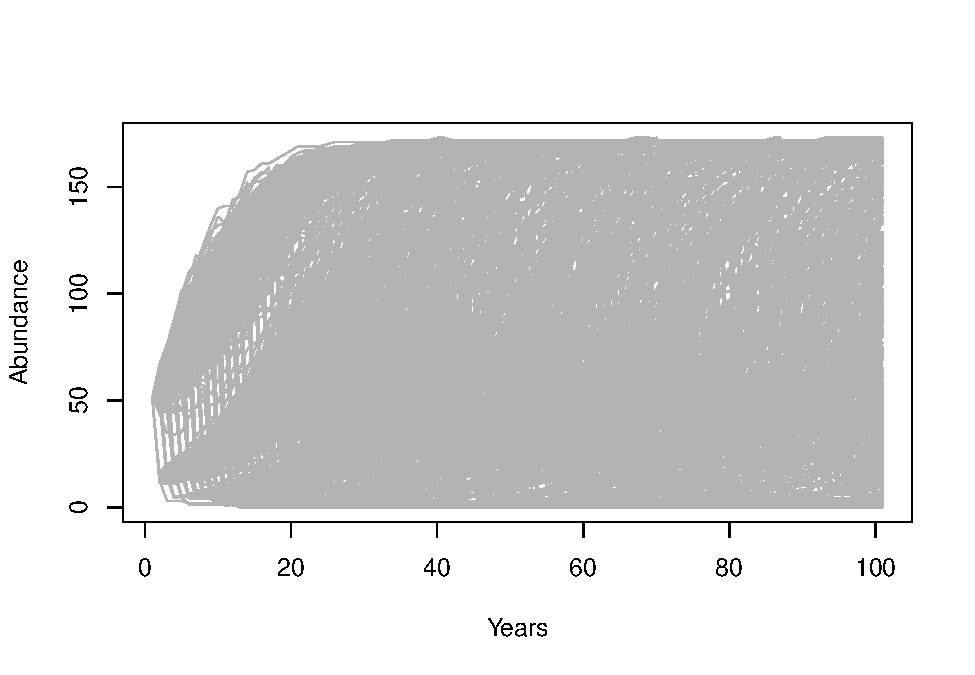
\includegraphics{LECTURE12_files/figure-latex/unnamed-chunk-4-1.pdf}

Bien, ¿qué aprendemos de esto? Realmente, es un desastre !!!

Si nuestra pregunta es sobre el riesgo de extinción, tal vez queramos
trazar el riesgo de extinción por tiempo \ldots{}

\begin{Shaded}
\begin{Highlighting}[]
\CommentTok{\# Visualice las tasas de extinción a lo largo del tiempo}

\NormalTok{Extinction\_byyear }\OtherTok{\textless{}{-}} \ControlFlowTok{function}\NormalTok{(simdata)\{}
  \FunctionTok{apply}\NormalTok{(simdata,}\DecValTok{1}\NormalTok{,}\ControlFlowTok{function}\NormalTok{(t)  }\FunctionTok{length}\NormalTok{(}\FunctionTok{which}\NormalTok{(t}\SpecialCharTok{==}\DecValTok{0}\NormalTok{)))}\SpecialCharTok{/}\FunctionTok{ncol}\NormalTok{(simdata)}
\NormalTok{\}}

\FunctionTok{plot}\NormalTok{(}\FunctionTok{c}\NormalTok{(}\DecValTok{1}\SpecialCharTok{:}\DecValTok{101}\NormalTok{),}\FunctionTok{Extinction\_byyear}\NormalTok{(Default),}\AttributeTok{type=}\StringTok{"l"}\NormalTok{,}\AttributeTok{lwd=}\DecValTok{2}\NormalTok{,}\AttributeTok{xlab=}\StringTok{"year"}\NormalTok{,}\AttributeTok{ylab=}\StringTok{"extinction risk"}\NormalTok{)}
\FunctionTok{abline}\NormalTok{(}\AttributeTok{h=}\FloatTok{0.05}\NormalTok{,}\AttributeTok{col=}\StringTok{"red"}\NormalTok{,}\AttributeTok{lwd=}\DecValTok{2}\NormalTok{)}
\end{Highlighting}
\end{Shaded}

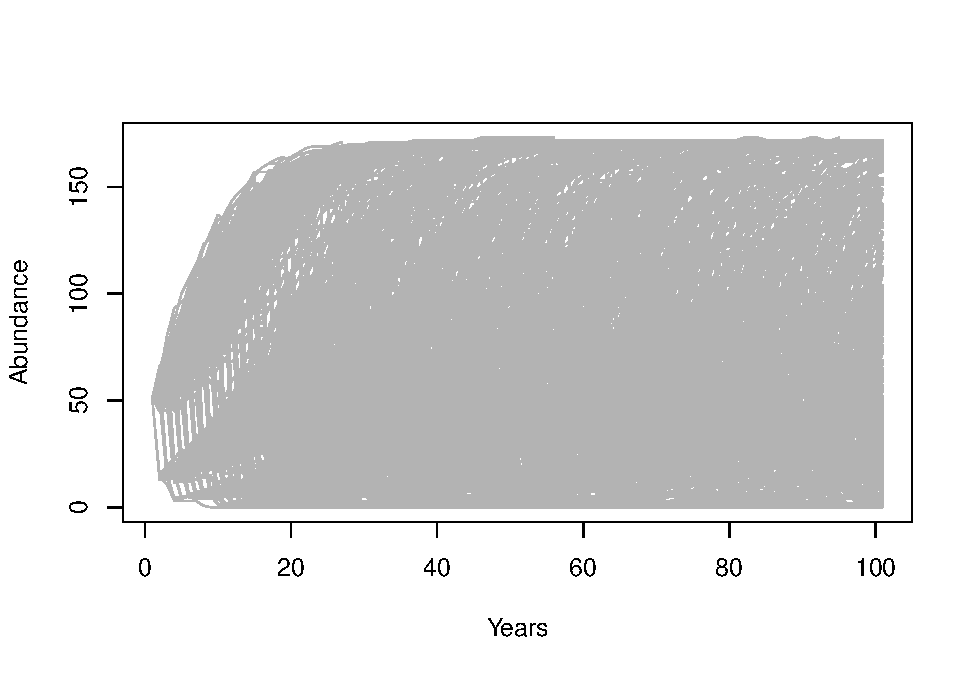
\includegraphics{LECTURE12_files/figure-latex/unnamed-chunk-5-1.pdf}

Quizás nuestra pregunta sea sobre la probabilidad de declive en 100 años
\ldots{}

En ese caso quizás deberíamos presentar un histograma de abundancias
finales \ldots{}

\begin{Shaded}
\begin{Highlighting}[]
\CommentTok{\# visualizar la abundancia final después de 100 años en relación con la abundancia inicial}

\FunctionTok{hist}\NormalTok{(Default[}\FunctionTok{nrow}\NormalTok{(Default),],}\AttributeTok{xlab=}\StringTok{"Final abundance after 100 years"}\NormalTok{,}\AttributeTok{ylab=}\StringTok{"Number of replicates"}\NormalTok{,}\AttributeTok{main=}\StringTok{""}\NormalTok{)}
\FunctionTok{abline}\NormalTok{(}\AttributeTok{v=}\NormalTok{Init\_N,}\AttributeTok{col=}\StringTok{"green"}\NormalTok{,}\AttributeTok{lwd=}\DecValTok{2}\NormalTok{)}
\end{Highlighting}
\end{Shaded}

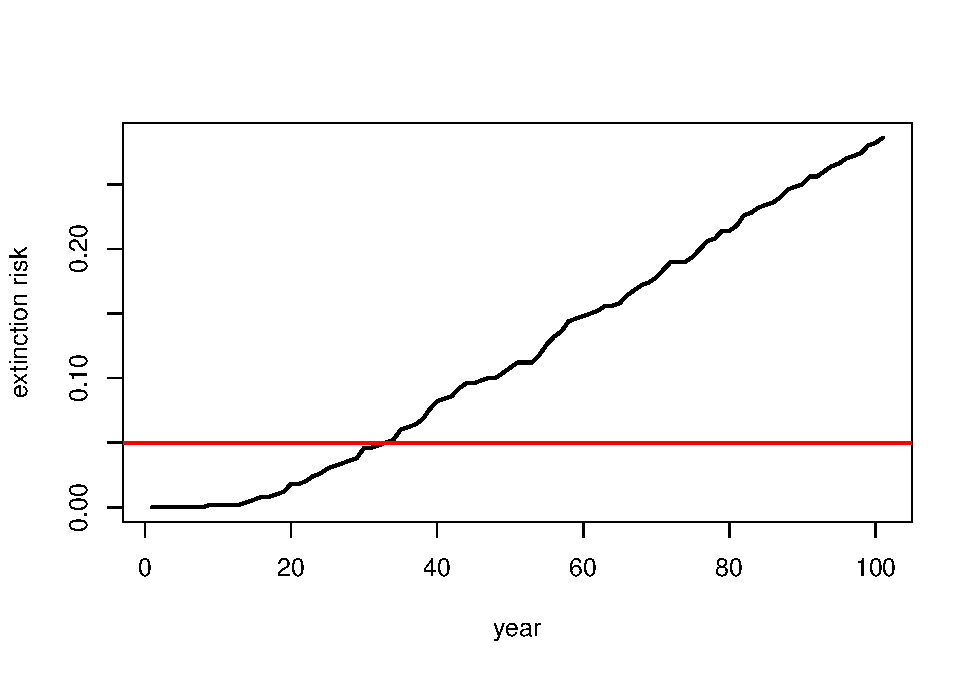
\includegraphics{LECTURE12_files/figure-latex/unnamed-chunk-6-1.pdf}

O podríamos graficar el grado de disminución frente a la probabilidad de
caer por debajo de ese umbral en el año 100.

\begin{Shaded}
\begin{Highlighting}[]
\CommentTok{\# plot probabilities of different severities of declinegraficar las probabilidades de diferentes grados de declive}

\NormalTok{declines }\OtherTok{\textless{}{-}} \FunctionTok{seq}\NormalTok{(}\DecValTok{0}\NormalTok{,}\DecValTok{100}\NormalTok{,}\AttributeTok{by=}\DecValTok{1}\NormalTok{)}
\NormalTok{declineprob }\OtherTok{\textless{}{-}} \FunctionTok{numeric}\NormalTok{(}\FunctionTok{length}\NormalTok{(declines))}

\ControlFlowTok{for}\NormalTok{(s }\ControlFlowTok{in} \DecValTok{1}\SpecialCharTok{:}\FunctionTok{length}\NormalTok{(declines))\{}
\NormalTok{  declineprob[s] }\OtherTok{\textless{}{-}} \FunctionTok{length}\NormalTok{(}\FunctionTok{which}\NormalTok{(Default[}\FunctionTok{nrow}\NormalTok{(Default),]}\SpecialCharTok{\textless{}}\NormalTok{(Init\_N}\SpecialCharTok{{-}}\NormalTok{(declines[s]}\SpecialCharTok{/}\DecValTok{100}\NormalTok{)}\SpecialCharTok{*}\NormalTok{Init\_N)))}\SpecialCharTok{/}\FunctionTok{ncol}\NormalTok{(Default)}
\NormalTok{\}}

\FunctionTok{plot}\NormalTok{(declines,declineprob,}\AttributeTok{type=}\StringTok{"l"}\NormalTok{,}\AttributeTok{lwd=}\DecValTok{2}\NormalTok{,}\AttributeTok{xlab=}\StringTok{"Decline threshold (percent)"}\NormalTok{,}\AttributeTok{ylab=}\StringTok{"Probability of falling below threshold"}\NormalTok{)}

\FunctionTok{abline}\NormalTok{(}\AttributeTok{v=}\DecValTok{25}\NormalTok{,}\AttributeTok{col=}\StringTok{"red"}\NormalTok{,}\AttributeTok{lwd=}\DecValTok{2}\NormalTok{)}
\end{Highlighting}
\end{Shaded}

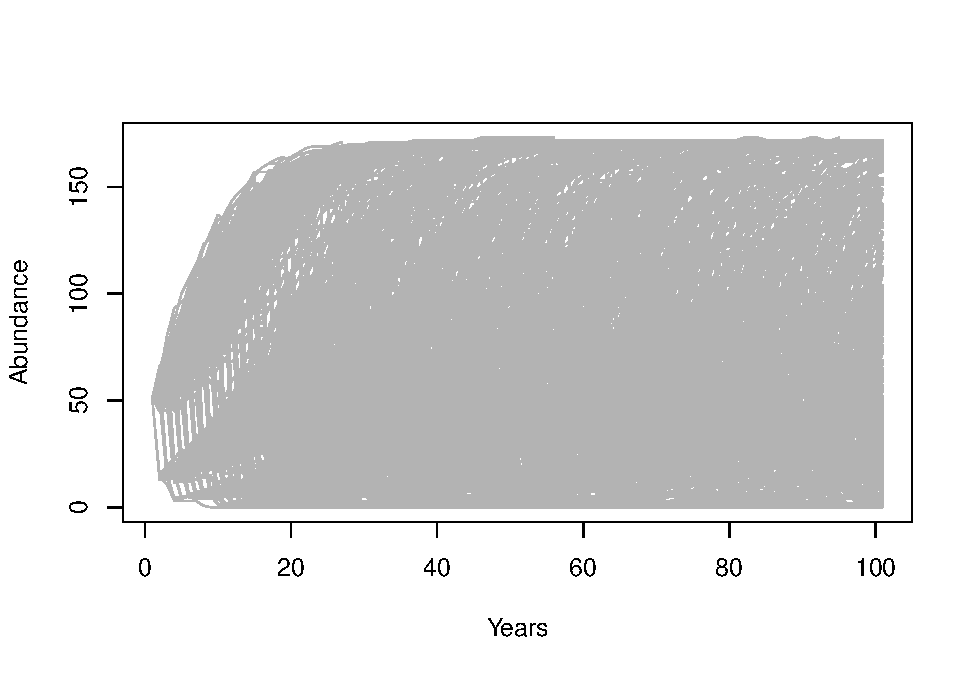
\includegraphics{LECTURE12_files/figure-latex/unnamed-chunk-7-1.pdf}

¿Y si nuestra pregunta es sobre el efecto de las inundaciones en el
riesgo de extinción? Imaginemos que no se espera que la probabilidad de
inundaciones cambie con el cambio climático, ¡pero es probable que la
intensidad de los daños por inundaciones aumente sustancialmente!

Actualmente, las inundaciones generalmente resultan en una reducción de
la población del 10\%. Pero el cambio climático podría aumentar este
número hasta en un 90\%. ¡Veamos cuánto podría aumentar esto el riesgo
de extinción!

\begin{Shaded}
\begin{Highlighting}[]
\CommentTok{\# Grafique el riesgo de extinción en función de la gravedad de las inundaciones}

\NormalTok{Exctinction\_risk }\OtherTok{\textless{}{-}} \ControlFlowTok{function}\NormalTok{(simdata)\{}
  \FunctionTok{length}\NormalTok{(}\FunctionTok{which}\NormalTok{(simdata[}\FunctionTok{nrow}\NormalTok{(simdata),]}\SpecialCharTok{==}\DecValTok{0}\NormalTok{))}\SpecialCharTok{/}\FunctionTok{ncol}\NormalTok{(simdata)}
\NormalTok{\}}

\NormalTok{flood\_lambdas }\OtherTok{\textless{}{-}} \FunctionTok{seq}\NormalTok{(}\FloatTok{0.9}\NormalTok{,}\FloatTok{0.1}\NormalTok{,}\AttributeTok{by=}\SpecialCharTok{{-}}\FloatTok{0.05}\NormalTok{)}

\NormalTok{all\_scenarios }\OtherTok{\textless{}{-}} \FunctionTok{numeric}\NormalTok{(}\FunctionTok{length}\NormalTok{(flood\_lambdas))}
\ControlFlowTok{for}\NormalTok{(scenario }\ControlFlowTok{in} \DecValTok{1}\SpecialCharTok{:}\FunctionTok{length}\NormalTok{(flood\_lambdas))\{}
\NormalTok{  PVA }\OtherTok{\textless{}{-}} \FunctionTok{PVAdemo}\NormalTok{(nreps,nyears,Init\_N,R\_max,K,Flood\_prob,flood\_lambdas[scenario])}
\NormalTok{  all\_scenarios[scenario] }\OtherTok{\textless{}{-}} \FunctionTok{Exctinction\_risk}\NormalTok{(PVA)}
\NormalTok{\}}

\FunctionTok{plot}\NormalTok{(flood\_lambdas,all\_scenarios,}\AttributeTok{type=}\StringTok{"p"}\NormalTok{,}\AttributeTok{cex=}\DecValTok{2}\NormalTok{,}\AttributeTok{xlab=}\StringTok{"flood impact (lambda in flood year)"}\NormalTok{,}\AttributeTok{ylab=}\StringTok{"extinction risk"}\NormalTok{)}
\FunctionTok{abline}\NormalTok{(}\AttributeTok{h=}\FloatTok{0.05}\NormalTok{,}\AttributeTok{col=}\StringTok{"red"}\NormalTok{,}\AttributeTok{lwd=}\DecValTok{2}\NormalTok{)}
\end{Highlighting}
\end{Shaded}

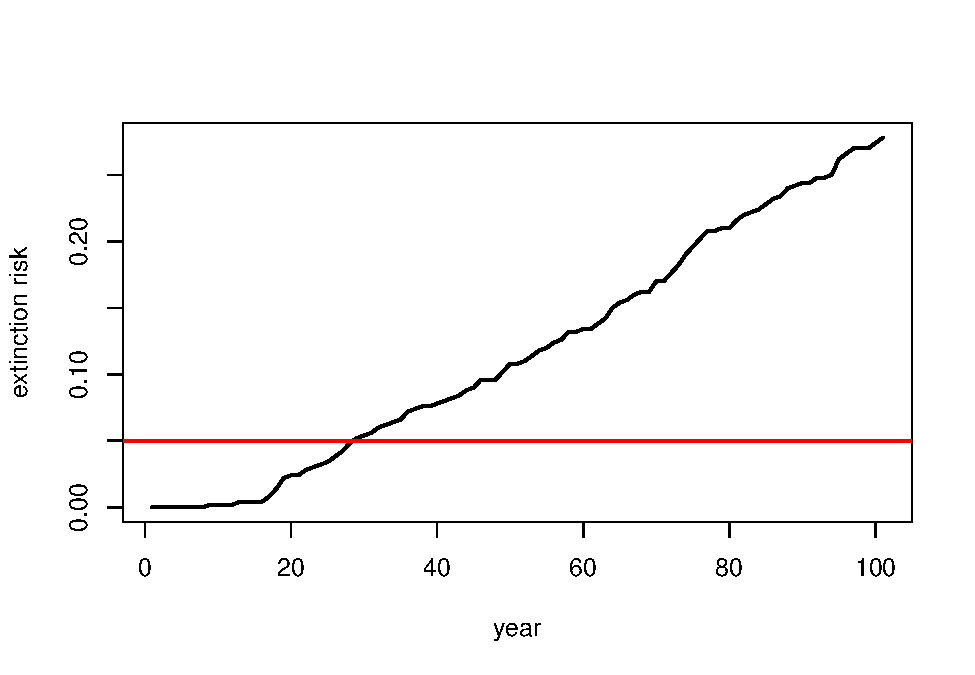
\includegraphics{LECTURE12_files/figure-latex/unnamed-chunk-8-1.pdf}

\href{LECTURE13.html}{--go to next lecture--}

\end{document}
